

\chapter{Subject of the thesis}
Building Chess AI is very difficult and time consuming process if it is require to achieve good effectiveness. In scope of this thesis an approach has been used that includes the following components:
\begin{itemize}
	\item game tree as an decision making structure,
	\item min-max algorithm as an search algorithm,
	\item game tree depth limit as an optimization method,
	\item artificial neural network as an first evacuation function,
	\item convolutional neural network as an second evaluation function.
\end{itemize}

\section{Decision making system - implementation}
Starting game tree structure is generated at the beginning of the program using recursive method. At the beginning of the program, there is option to choose game tree depth limit. This configuration specify how many moves needs to be included in game tree structure. When last layer of the structure will be achieved, game tree will be destroyed and regenerated with the same depth. As it was described in section \ref{sec:game-tree-optimizations}, it is impossible to generate full game tree of chess, so that is why game tree depth limitation has been used. The most commonly used game tree depth limit is $3$. It is possible to specify different value of this parameter but it is important to keep in mind that it will impact time needed to make decision. Example structure of game tree used in the the project can be seen on \hyperref[fig:game-tree-fragment]{fig.  \ref*{fig:game-tree-fragment}}.
\begin{figure}
	\centering
	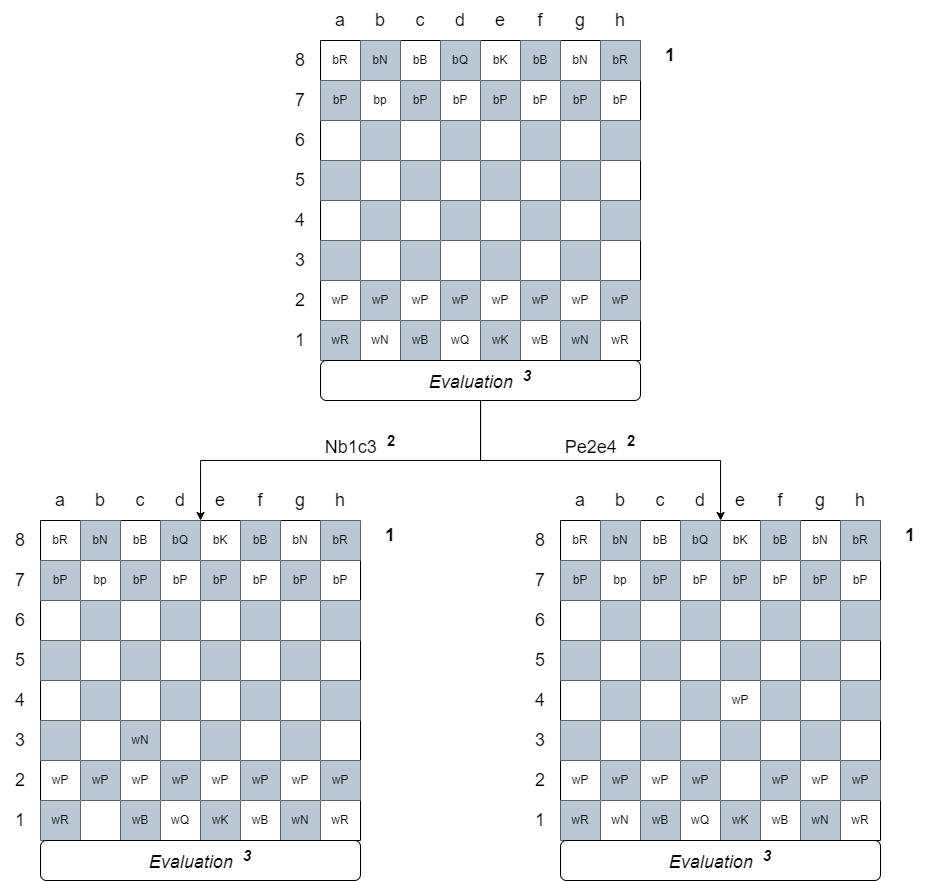
\includegraphics[width=\textwidth]{dependencies/pictures/Game_Tree_Fragment_Example.png}
	\caption{Game tree fragment example (1 - chess board representation, 2 - move command, 3 - evaluation value).}
	\label{fig:game-tree-fragment}
\end{figure}

Created game tree is used as an input to the min-max search algorithm. Detail explanation of this algorithm can be found in section \ref{sec:min-max-algorithm}. There are 2 main assumptions that needs to be explain while describing usage of min-max algorithm in scope of this thesis. If game take place in scenario ,,player vs AI'', human player always is assign to white site of the board which also result in making first move. If game scenario is set to be ,,AI vs AI'', each of the instances gets assign randomly to one of the site. Sequence in which min-max algorithm work can be specified as follows:
\begin{enumerate}
	\item Find the most beneficial sequence of moves in generated game tree.
	\item Get chessboard situation after opponents move.
	\item If gathered node is not one of game tree nodes, go back to point 1. Otherwise, regenerate game tree and go back to point 1.
\end{enumerate}
Important thing to mentioned is the fact that in scope of this thesis there are no optimization method used for min-max algorithm. It can result in increasing time of making decisions while playing. It was decided to use min-max tree structure because it is core element of a lot of other chess playing AI and it it the mos beneficial solution. 

\section{Evaluation system - implementation}
To make all experiments more accurate, it ha been decided to implement very basic models of ANN and CNN. To increase accuracy even more, both instances were coded from scratch and trained on the same datasets. Using neural network model as an evaluation method is not a new approach but usage of CNN and ANN, on the other hand is, because the most often used models are genetic algorithm based one. It is hard to predict how effective this approach would be, before analyzing tests results, but it can be very interesting how it perform. 

Before further discursion it is necessary to describe how chessboard is represented in the final program. There are $3$ methods that chess pieces are stored: number type, string type and object type. All of those types are shown in \hyperref[tab:chess-pieces-types]{tab. \ref*{tab:chess-pieces-types}} (object type will be skipped in the table).
\begin{table}
	\centering
	\caption{The list of chess pieces types.}
	\label{tab:chess-pieces-types}
	\begin{tabular}{ccc}
	\toprule
		\textbf{symbol} & \textbf{number value} & \textbf{string value}\\
		\hline
			\WhiteKingOnWhite \BlackKingOnWhite & 7 / -7 & wK / bK\\
		\hline
			\WhiteQueenOnWhite \BlackQueenOnWhite & 5 / -5 & wQ / bQ\\
		\hline
			\WhiteBishopOnWhite \BlackBishopOnWhite & 4 / -4 & wB / bB\\
		\hline
			\WhiteKnightOnWhite \BlackKnightOnWhite & 3 / -3 & wN / bN\\
		\hline
			\WhiteRookOnWhite \BlackRookOnWhite & 2 / -2 & wR / bR\\
		\hline
			\WhitePawnOnWhite \BlackPawnOnWhite & 1 / -1 & wP / bP\\
	\end{tabular}
\end{table}
Data structure containing numerical values representing chess pieces will be used as an input in both instances of created neural networks.

\subsection{Artificial neural network - architecture}
As it was mentioned before, each of neural network instances was implemented from scratch to make experiments more reliable. When creating artificial neural network instance, there are two main aspects that needs to be specified. First and the most crucial topic is to design architecture of the network. Because problem that needs to be solved is evaluating chessboard situation, created network needs to take $64$ values as an input (chessboard have dimension of $8 \times 8$) and needs to return one value which will be assigned as an evaluation value to the specific chessboard situation. To keep created model as simple as possible, it has been decided to include only two hidden layers with $64$ neurons each. When structure of the network has been created, there is one last important configuration to establish. As it was mentioned in section \ref{sec:learning-process-for-nn-instance}, every instance of neural network needs to have learning rate parameter specified. During training process, it was established that learning rate value for artificial neural network should be equal to $0.001$. This value resulted in the most efficient training process for this model. It is possible that ANN evaluation function will not provide spectacular results for given problem but it is important to remember that it has been used as an basic point of comparison for second evaluation. This method allows to decide if usage of CNN, for evaluating chessboard situations, is an justified or beneficial solution to the problem.

\subsection{Convolutional neural network - architecture}
While planing structure for convolutional neural network, the main goal was to keep structure of the model simple. This decision has been made because if basic structure of CNN model won't perform better than basic structure of ANN, it is a proof that given solution is bad. Second reason for keeping model structure simple is less time consuming training process for both models. There are two elements in convolutional neural network configuration that are similar to the first used model. The best value for learning rate parameter is equal to $0.001$ and sizes of input and output layers are also the same like in artificial neural network. It has been decided that CNN model will consists of two convolutional layers, with 13 and 10 kernels respectively, two pooling layers, two activation layers and one fully connected layer. Full structure of the used CNN can be found on \hyperref[fig:cnn-structure]{fig. \ref*{fig:cnn-structure}}.
\begin{figure}
	\centering
	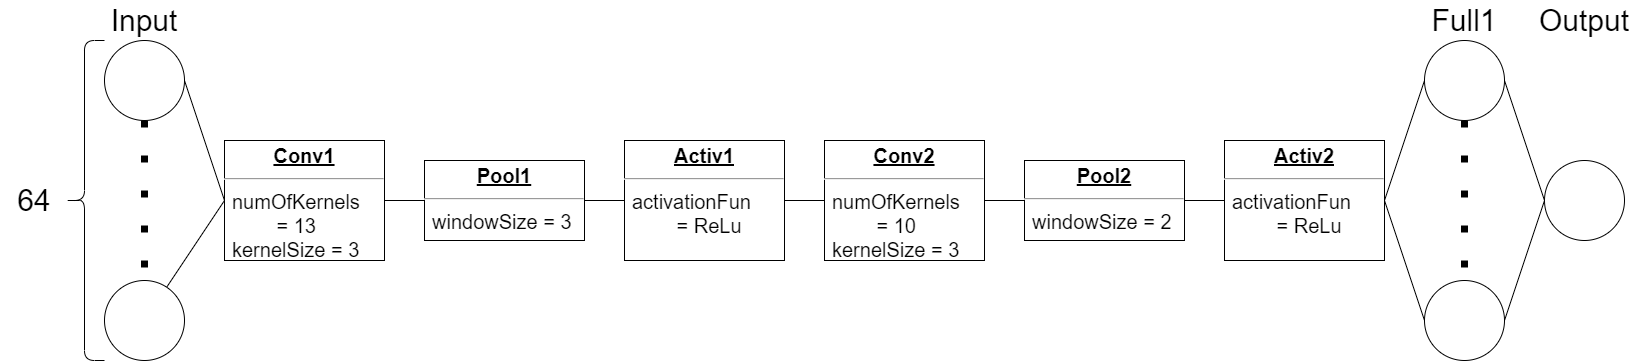
\includegraphics[width=\textwidth]{dependencies/pictures/CNN_Structure.png}
	\caption{Structure of the implemented CNN.}
	\label{fig:cnn-structure}
\end{figure}
In the contrary to ANN hidden layers, which number of neurons are not backed by any theoretical aspects, convolutional layers was design based on chess game theory. According to publications about chess there are $13$ the best openings which give player the most benefits. This is why first convolutiona layer consists of $13$ kernels. Second convolutional layer consists of $10$ kernels because this is the number of the most commonly used, beneficial chessboard arrangements \cite{bib:book-mastering-chess-logic,bib:book-chess-bible,bib:book-bobby-fisher-teaches-chess}. The assumption is that both convolutional layers will be responsible for detecting mentioned chessboard arrangements.

\section{Used tools}
In the scope this thesis, all components of the final project has been implemented from scratch using C++17 language. As an IDE Visual Studio Code (VSCode) has been chosen. To build and prepare project for compilation Premake software has been used. This thesis has been written using \LaTeX language and VSCode IDE. For creating all diagrams used in this thesis, Draw.io online software has been used. In the creative process of this project, the sources included in the bibliography and following documentations were used: \cite{bib:internet-c++-doc,bib:internet-latex-doc,bib:internet-vscode-doc,bib:internet-premake-doc}.

% tekst

% \section{[Section title]}

% \section{[Subsection title]}

% Each figure in the document should be referred to at least once (fig. \ref{fig:2}).

% \begin{figure}
% \centering
% \begin{tikzpicture}
% \begin{axis}[
%     y tick label style={
%         /pgf/number format/.cd,
%             fixed,   % po zakomentowaniu os rzednych jest indeksowana wykladniczo
%             fixed zerofill, % 1.0 zamiast 1
%             precision=1,
%         /tikz/.cd
%     },
%     x tick label style={
%         /pgf/number format/.cd,
%             fixed,
%             fixed zerofill,
%             precision=2,
%         /tikz/.cd
%     }
% ]
% \addplot [domain=0.0:0.1] {rnd};
% \end{axis} 
% \end{tikzpicture}
% \caption{Figure caption.} % Figure caption is BELOW the figure!
% \label{fig:2}
% \end{figure}

% Each table in the document should be referred to at least once (Tab. \ref{tab:results}).

% \begin{table}
% \centering
% \caption{A caption of a table is ABOVE it.}
% \label{tab:results}
% \begin{tabular}{rrrrrrrr}
% \toprule
% 	         &                                     \multicolumn{7}{c}{method}                                      \\
% 	         \cmidrule{2-8}
% 	         &         &         &        \multicolumn{3}{c}{alg. 3}        & \multicolumn{2}{c}{alg. 4, $\gamma = 2$} \\
% 	         \cmidrule(r){4-6}\cmidrule(r){7-8}
% 	$\zeta$ &     alg. 1 &   alg. 2 & $\alpha= 1.5$ & $\alpha= 2$ & $\alpha= 3$ &   $\beta = 0.1$  &   $\beta = -0.1$ \\
% \midrule
% 	       0 &  8.3250 & 1.45305 &       7.5791 &    14.8517 &    20.0028 & 1.16396 &                       1.1365 \\
% 	       5 &  0.6111 & 2.27126 &       6.9952 &    13.8560 &    18.6064 & 1.18659 &                       1.1630 \\
% 	      10 & 11.6126 & 2.69218 &       6.2520 &    12.5202 &    16.8278 & 1.23180 &                       1.2045 \\
% 	      15 &  0.5665 & 2.95046 &       5.7753 &    11.4588 &    15.4837 & 1.25131 &                       1.2614 \\
% 	      20 & 15.8728 & 3.07225 &       5.3071 &    10.3935 &    13.8738 & 1.25307 &                       1.2217 \\
% 	      25 &  0.9791 & 3.19034 &       5.4575 &     9.9533 &    13.0721 & 1.27104 &                       1.2640 \\
% 	      30 &  2.0228 & 3.27474 &       5.7461 &     9.7164 &    12.2637 & 1.33404 &                       1.3209 \\
% 	      35 & 13.4210 & 3.36086 &       6.6735 &    10.0442 &    12.0270 & 1.35385 &                       1.3059 \\
% 	      40 & 13.2226 & 3.36420 &       7.7248 &    10.4495 &    12.0379 & 1.34919 &                       1.2768 \\
% 	      45 & 12.8445 & 3.47436 &       8.5539 &    10.8552 &    12.2773 & 1.42303 &                       1.4362 \\
% 	      50 & 12.9245 & 3.58228 &       9.2702 &    11.2183 &    12.3990 & 1.40922 &                       1.3724 \\
% \bottomrule
% \end{tabular}
% \end{table}  


%\chapter{[Subject of the thesis]}
%
%\begin{itemize}
%\item solution to the problem proposed by the author of the thesis
%\item theoretical analysis of proposed solutions
%\item rationale of applied methods, algorithms, and tools
%\end{itemize}